\documentclass[11pt,a4paper]{article}
\usepackage[T1]{fontenc}
\usepackage{lmodern}
\usepackage[margin=23mm]{geometry}
\usepackage{amsmath,amssymb}
\usepackage{xcolor}
\usepackage{tikz}
\usetikzlibrary{arrows.meta,positioning,calc}
\usepackage{hyperref}
\hypersetup{colorlinks=true,linkcolor=blue!45!black,urlcolor=blue!45!black}
\setlength{\parindent}{0pt}
\setlength{\parskip}{5pt plus 1pt}
\setlength{\emergencystretch}{2em}
\definecolor{water}{RGB}{205,231,241}
\definecolor{ink}{RGB}{30,62,79}
\tikzset{flow/.style={-{Latex},thick,ink}, equipment/.style={thick,ink},
         box/.style={draw=ink,rounded corners,align=center,inner sep=5pt}}
\title{Intelligent Systems for Process Control and Automation\\[4pt]{\large Eight connected study units}}
\author{Independent study collection}
\date{}
\begin{document}
\maketitle
\noindent Academic context: Intelligent Systems for Process Control and Automation, Prof. Michela Mulas. These newly written learning materials are not an official course plan and do not imply the professor's authorship, review or endorsement.

\tableofcontents\newpage
\clearpage\section{Unit 01: Modeling, identification and simulation}
\textbf{Prerequisites:} Differential equations, units, matrix least squares and elementary probability.

\begin{center}
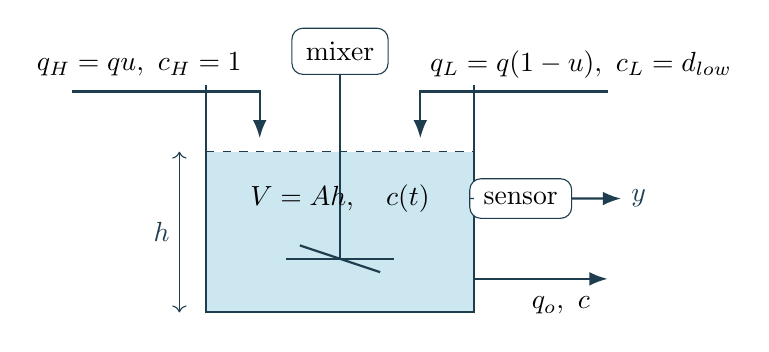
\begin{tikzpicture}[scale=0.85]
\fill[water] (0,0) rectangle (4,2.4);
\draw[equipment] (0,3.4)--(0,0)--(4,0)--(4,3.4);
\draw[ink,dashed] (0,2.4)--(4,2.4);
\draw[flow] (-2,3.3)--(0.8,3.3)--(0.8,2.6);
\draw[flow] (6,3.3)--(3.2,3.3)--(3.2,2.6);
\draw[flow] (4,0.5)--(6,0.5);
\draw[equipment] (2,3.8)--(2,0.8);
\draw[equipment] (1.2,0.8)--(2.8,0.8);
\draw[equipment] (1.4,1.0)--(2.6,0.6);
\node[box,fill=white] at (2,3.9) {mixer};
\node at (-1,3.7) {$q_H=qu,\ c_H=1$};
\node at (5.6,3.7) {$q_L=q(1-u),\ c_L=d_{low}$};
\node at (5.3,0.1) {$q_o,\ c$};
\node at (2,1.7) {$V=Ah,\quad c(t)$};
\draw[<->,ink] (-0.4,0)--node[left] {$h$}(-0.4,2.4);
\node[box,fill=white] (sensor) at (4.7,1.7) {sensor};
\draw[ink] (4,1.7)--(sensor);
\draw[flow] (sensor.east)--(6.2,1.7) node[right] {$y$};
\end{tikzpicture}
\end{center}
\noindent\textit{Physical boundary for the analytical tank. A constant-volume model requires inlet and outlet balance. Here the disturbance is low-feed concentration; the shared laboratory instead uses an additive disturbance to the complete inlet mixture. The sensor reading may have dynamics distinct from concentration.}

\subsection{A model begins with a boundary}

A controller changes a physical input; its software output is not automatically that input. Draw the vessel, inlet streams, outlet, sensor and valve before naming states. For a perfectly mixed tank with constant density and cross-sectional area $A$, conservation gives


\[A\dot h=q_H+q_L-q_o,\qquad \frac{d(Ahc)}{dt}=q_Hc_H+q_Lc_L-q_oc.\]

Expanding the derivative and substituting the volume balance cancels the outlet term in the concentration equation:


\[\dot c=\frac{q_H(c_H-c)+q_L(c_L-c)}{Ah}.\]

This cancellation does not mean the outlet is irrelevant: it changes $h$, which changes the residence time. Mixing is assumed instantaneous; density differences, reaction, evaporation and sensor dynamics are absent. A simulation approaching $h=0$ must stop or change its physical model rather than divide by a clipped volume silently.


\subsection{A common worked process}

The exercises use hypothetical values $V=100$ L, total flow $q=10$ L/min and normalized feed concentrations $c_H=1$, $c_L=0$. A low-level flow system holds $q$ constant while $q_H=qu$ and $q_L=q(1-u)$, with $0\leq u\leq1$. Thus


\[\tau\dot c=u-c,\qquad \tau=V/q=10\ {\rm min}.\]

These are new teaching parameters, not a transcription of the archived Blending Tank files. At a constant input, $c^*=u^*$. In deviation variables, $G(s)=1/(10s+1)$. At a one-minute sampling period with a zero-order-held input,


\[c_{k+1}=ac_k+bu_k,\qquad a=e^{-0.1}=0.904837418,\quad b=1-a=0.095162582.\]

The analytical feed-composition problems use $d=d_{low}$ for the concentration of the low feed, giving an inlet mixture $u+(1-u)d_{low}$. The shared executable laboratory scenario instead uses an additive disturbance to the total inlet mixture, $u+d_{mix}$. Their conversion is $d_{mix}=(1-u)d_{low}$, so they are not interchangeable at fixed numerical values. Feedforward in the additive scenario compensates by $-d_{mix}$; the low-feed examples derive the nonlinear blend formula explicitly. Check the disturbance definition before comparing a worked answer with a laboratory run.


The exact discretization preserves the interval $[0,1]$ because the next concentration is a convex combination of the current concentration and the inlet blend. Forward Euler gives $a_E=1-T_s/\tau$; it is asymptotically stable for $0<T_s<2\tau$ but preserves this physical interval only for $0<T_s\leq\tau$.


\subsection{Identification is an experiment-design problem}

Fit $y_{k+1}=ay_k+bu_k+e_{k+1}$ by least squares, $\hat\theta=(\Phi^T\Phi)^{-1}\Phi^TY$, only when the regressor matrix has full column rank. In software, use a QR/SVD least-squares solve rather than forming the inverse. A constant equilibrium record cannot identify both coefficients. Step tests help, but a bounded multilevel or persistently exciting signal gives a broader operating region.


Split complete trajectories chronologically into training, validation and final test sets. Fit scaling parameters on training data only. A one-step prediction uses the measured previous output; free simulation recursively uses its own prediction. Report both because a small one-step error can hide unstable recursive behavior. With noisy measured regressors, ordinary least squares can be biased; instrumental variables or a noise model may be needed.


\subsection{Evidence and interpretation}

Check mass conservation, equilibria, convergence when the integration step is halved, and agreement with the analytical step response. Inspect residual autocorrelation and correlation with past inputs on an independent trajectory. Residual whiteness alone does not prove a correct physical model. Use the benchmark inventory to distinguish equation-based simulations from experimental datasets, and do not compare numerical scores obtained with different input protocols as if they were the same experiment.

\clearpage\section{Unit 02: Feedback, stability and IMC tuning}
\textbf{Prerequisites:} Unit 01; Laplace transforms, characteristic polynomials and negative feedback.

\subsection{Separate the plant, controller and actuator}

For the hypothetical tank $P(s)=1/(\tau s+1)$, define the tracking error $e=r-y$ and a PI command $v=K_pe+I$, with $\dot I=K_ie$. The applied blend is $u=\operatorname{sat}_{[0,1]}(v)$. A control diagram that omits this saturation cannot explain windup. For a PID controller, differentiate a filtered measurement rather than an abrupt reference when derivative kick is undesirable; for example use $-K_ds/(1+T_fs)$ on $y$.


With ideal measurement, no saturation and PI feedback, the closed-loop characteristic polynomial is


\[\tau s^2+(1+K_p)s+K_i.\]

The second-order continuous model is asymptotically stable when $\tau>0$, $1+K_p>0$ and $K_i>0$. This result does not cover delays, sampled implementation or saturating nonlinear dynamics. The final-value theorem also requires a stable closed loop before it can justify zero constant-reference error.


\subsection{Derive an IMC design rather than memorize gains}

For the stable minimum-phase model $\hat P=1/(\tau s+1)$, choose $Q=(\tau s+1)/(\lambda s+1)$. Converting the internal-model structure to ordinary feedback gives


\[C=\frac{Q}{1-\hat P Q}=\frac{\tau s+1}{\lambda s},\qquad K_p=\frac{\tau}{\lambda},\quad K_i=\frac1\lambda.\]

Nominal pole-zero cancellation makes $Y/R=1/(\lambda s+1)$, but the canceled pole still matters to internal dynamics and mismatch. With $\tau=10$ min and $\lambda=5$ min, $K_p=2$ and $K_i=0.2$ per minute. For a first-order-plus-dead-time approximation, the commonly used IMC-PI rule $K_p=\tau/[K(\lambda+\theta)]$, $T_i=\tau$ trades speed for delay tolerance; it is an approximation, not exact cancellation of a delay.


\subsection{Implement the controller that was analyzed}

One explicit digital update is $v_k=K_pe_k+I_k$, $u_k=\operatorname{sat}(v_k)$, then $I_{k+1}=I_k+T_s[K_ie_k+K_{aw}(u_k-v_k)]$. Here $K_{aw}$ has units of inverse time because $I$ has actuator units. Conditional integration is another option: freeze integration when saturation and the error would push farther into the limit. Keep update order and derivative state explicit in MATLAB, Octave and Python.


The local discrete closed-loop matrix for the unsaturated explicit update and zero reference is


\[M=\begin{bmatrix}a-bK_p&b\\-T_sK_i&1\end{bmatrix}.\]

Its eigenvalues, not continuous poles alone, determine sampled stability. A reference beyond the attainable concentration range has no feasible equilibrium, however stable the local model is.


\subsection{Compare outcomes on the same experiment}

Use identical initial state, reference steps, feed disturbances and actuator limits. Record tracking error, settling definition, total variation $\sum|u_k-u_{k-1}|$, saturation time and any violation. A smoother input may be valuable even if its integral absolute error is larger. Disturbance rejection and sensor-noise amplification are distinct design goals; one appealing tracking plot cannot demonstrate both.

\clearpage\section{Unit 03: Multiloop, multivariable, feedforward and cascade control}
\textbf{Prerequisites:} Units 01-02; matrix inversion and local transfer functions.

\begin{center}
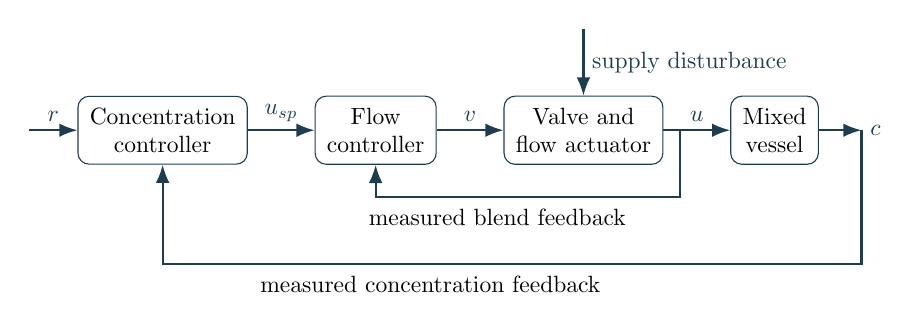
\begin{tikzpicture}[node distance=1.0cm,scale=0.85,transform shape]
\node[box] (outer) {Concentration\\controller};
\node[box,right=of outer] (inner) {Flow\\controller};
\node[box,right=of inner] (valve) {Valve and\\flow actuator};
\node[box,right=of valve] (tank) {Mixed\\vessel};
\draw[flow] (-2,0)--node[above] {$r$}(outer);
\draw[flow] (outer)--node[above] {$u_{sp}$}(inner);
\draw[flow] (inner)--node[above] {$v$}(valve);
\draw[flow] (valve)--node[above] {$u$}(tank);
\draw[flow] (tank)--++(1.3,0) coordinate (out) node[right] {$c$};
\draw[flow] ($(valve.east)+(0.25,0)$)--++(0,-1.0)-|(inner.south);
\draw[flow] (out)--++(0,-2)-|(outer.south);
\node at (5,-1.3) {measured blend feedback};
\node at (4,-2.3) {measured concentration feedback};
\draw[flow] ($(valve.north)+(0,1)$)--node[right] {supply disturbance}(valve.north);
\end{tikzpicture}
\end{center}
\noindent\textit{Cascade uses a measured inner variable. Both feedback paths are negative under the error conventions stated in the text.}

\subsection{Match architecture to the physical disturbance path}

Feedback acts after an output error is visible. Feedforward uses a measured disturbance before that error develops. For $10\dot c=u+(1-u)d-c$, holding the equilibrium at $r$ requires


\[u_{ff}=\frac{r-d}{1-d},\qquad d\ne1.\]

For $0\leq d<1$, this is feasible only when $d\leq r\leq1$. Feedback can trim errors in $d$, mixing and actuator calibration; it cannot repair an impossible target. The linear cancellation formula is $F(s)=-G_d(s)/G_u(s)$. A nonminimum-phase zero or unfavorable delay in $G_u$ can make the ideal inverse unstable or noncausal, so practical feedforward often uses a filtered approximation.


\subsection{Cascade closes a faster measured loop}

Suppose a valve command $v$ produces the actual blend $u$ through $\tau_v\dot u=v-u+w$, where $w$ is a valve/load disturbance. A fast inner controller regulates measured $u$ to an outer command $u_{sp}$; the outer concentration controller then sees the closed inner dynamics. With inner proportional gain $K_f$ and the feedforward equilibrium command $v=u_{sp}+K_f(u_{sp}-u)$, the inner pole is $-(1+K_f)/\tau_v$. A practical cascade needs an inner sensor, useful bandwidth separation and consistent actuator limits. A fast model is not evidence that an actual noisy valve can move arbitrarily quickly.


\subsection{Interactions require a joint view}

For a local steady two-input/two-output gain matrix $K$, the relative gain array is $\Lambda=K\circ(K^{-1})^T$, where $\circ$ denotes elementwise multiplication. For


\[K=\begin{bmatrix}1&0.6\\0.4&1\end{bmatrix},\qquad \Lambda=\begin{bmatrix}1.315789&-0.315789\\-0.315789&1.315789\end{bmatrix}.\]

Diagonal pairing avoids negative relative gains here. RGA is a local steady-state diagnostic, not a stability proof: dynamics, delays and operating-point changes still matter. Static decoupling $u=K^{-1}v$ removes steady interaction for the nominal model, but can demand infeasible or rapidly changing physical inputs. If saturation occurs, the assumed decoupling is lost.


\subsection{Compare architectures under matched conditions}

Start with independently tuned PI loops, then add measured-disturbance feedforward, cascade or decoupling for a stated reason. Keep the total available measurements explicit; a design with an additional disturbance sensor has an information advantage. Introduce one disturbance at a time, then simultaneous changes and model mismatch. Report output-by-output errors as well as a combined score. In Simulink, keep the physical plant, measurement path and controller subsystems separate so their responsibilities remain visible.

\clearpage\section{Unit 04: Constrained model predictive control}
\textbf{Prerequisites:} Units 01-03; quadratic forms, least squares and constrained optimization.

\begin{center}
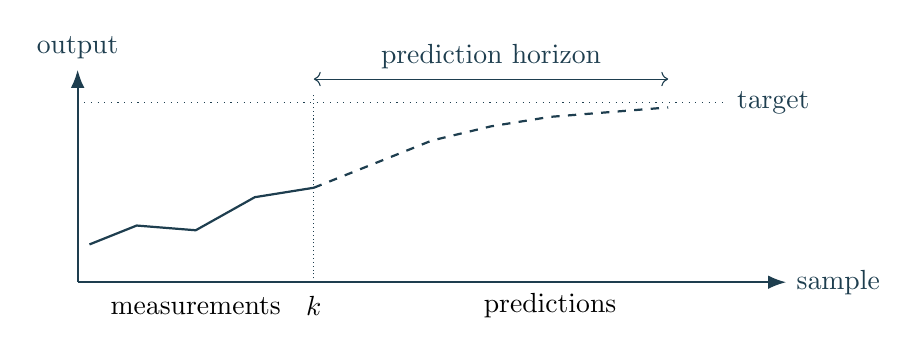
\begin{tikzpicture}[x=0.75cm,y=0.6cm]
\draw[flow] (0,0)--(12,0) node[right] {sample};
\draw[flow] (0,0)--(0,4.5) node[above] {output};
\draw[ink,thick] (0.2,0.8)--(1,1.2)--(2,1.1)--(3,1.8)--(4,2);
\draw[ink,dashed,thick] (4,2)--(5,2.5)--(6,3)--(7,3.3)--(8,3.5)--(9,3.6)--(10,3.7);
\draw[ink,densely dotted] (4,0)--(4,4);
\draw[ink,dotted] (0,3.8)--(11,3.8) node[right] {target};
\node at (2,-0.5) {measurements};
\node at (4,-0.5) {$k$};
\node at (8,-0.5) {predictions};
\draw[<->,ink] (4,4.3)--node[above] {prediction horizon}(10,4.3);
\end{tikzpicture}
\end{center}
\noindent\textit{The future curve is a model prediction, not an observed trajectory. Only the first planned input is applied before the next measurement.}

\subsection{Predict several steps, apply only the first action}

For $x_{k+1}=Ax_k+Bu_k$, $y_k=Cx_k$, assemble predicted outputs as $Y=Fx_k+GU$, where $U=[u_k^T,\ldots,u_{k+N-1}^T]^T$. The first block rows are $CA$ in $F$ and $CB$ in $G$; the second are $CA^2$ and $[CAB,CB]$. Use a consistent convention: these predictions begin at $k+1$.


A useful objective is


\[J=(Y-R)^TQ(Y-R)+(DU-d_0)^TR_u(DU-d_0),\]

where $DU-d_0$ stacks input increments and its first element is $u_k-u_{k-1}$. Bounds on $U$, input increments and predicted outputs become linear inequalities. Penalizing input magnitude instead of increments solves a different problem, especially around nonzero operating points. The Hessian is positive definite when the regularization supplies strictly positive curvature in every free input direction.


At each sample, estimate the state, solve the optimization, apply the first action, and repeat. Use a shorter control horizon by holding the last planned move constant; write this mapping explicitly rather than silently changing the prediction length. Log solver status, time and fallback use. A failed solver must not be treated as a valid optimum.


\subsection{One step exposes the tradeoff}

For $c^+=ac+bu$ and $J=(c^+-r)^2+\rho(u-u_{old})^2$, the unconstrained optimum is


\[u^*=\frac{b(r-ac)+\rho u_{old}}{b^2+\rho}.\]

With only scalar interval constraints, project this value onto their intersection. This is exact for the scalar one-step problem; independently clipping a general coupled multistep solution is not equivalent to solving its constrained quadratic program.


\subsection{Constraints and offset have different causes}

If the target lies beyond the attainable set, no horizon removes that incompatibility. Soften selected output targets with nonnegative slack and an explicit penalty when the application permits it; keep actuator bounds hard. For persistent model mismatch, augment a constant disturbance state and estimate it, or add another justified offset-free mechanism. A large prediction horizon alone does not guarantee zero steady error.


\subsection{Stability is a design property to establish}

Finite-horizon optimization and decreasing simulated error do not automatically imply closed-loop stability. Classical sufficient conditions involve suitable terminal cost, terminal invariant constraints and a feasible terminal controller. The teaching implementations demonstrate finite-horizon behavior under their declared experiments; do not infer a global nonlinear stability theorem. For multivariable processes, inspect individual output constraints and input allocation, not just the sum of squared errors.

\clearpage\section{Unit 05: Knowledge-based supervision and fuzzy control}
\textbf{Prerequisites:} Units 01-03; sets, piecewise functions and numerical integration.

\subsection{Supervisory rules express decisions and evidence}

A rule such as IF the concentration residual is large AND the flow sensor agrees with its command THEN suspect a concentration-path fault represents a diagnostic hypothesis. It does not prove a failed sensor. Store the measured evidence, persistence interval, action and reset condition separately. Use priorities for conflicting rules: an invalid measurement should inhibit a normal optimization request. Hysteresis and dwell time prevent repeated switching near a threshold. A low concentration alone cannot distinguish an inlet change, valve fault or concentration-sensor bias.


\subsection{Fuzzy membership is a degree of compatibility}

On a normalized error domain $[-1,1]$, define negative, zero and positive memberships by $\mu_N(e)=\max(0,-e)$, $\mu_Z(e)=1-|e|$ and $\mu_P(e)=\max(0,e)$, after explicitly limiting $e$ to the domain. They sum to one. These numbers are not probabilities unless a separate probabilistic interpretation is established. Input scaling determines which physical errors activate each rule.


For a two-input controller using error and error change, a rule might be IF error is positive AND error change is positive THEN increase the blend strongly. Specify whether AND is minimum or product. Mamdani inference clips or scales an output membership function for every firing rule, aggregates the results, and often defuzzifies with the centroid:


\[u_f=\frac{\int z\,\mu_{out}(z)\,dz}{\int\mu_{out}(z)\,dz}.\]

For zero-order Sugeno inference, singleton consequents $z_i$ give $u_f=(\sum_i w_i z_i)/(\sum_i w_i)$. This generally differs from the centroid of overlapping Mamdani sets. If no rule fires, use a documented fallback; adding an arbitrary epsilon to the denominator does not define a meaningful inference result.


\subsection{Fuzzy control can act at several levels}

A fuzzy controller may directly choose the command, produce its increment, or schedule PI/PID gains. If $u_k=u_{k-1}+K_u u_f$, then $K_u$ and the sampling interval determine how quickly the actuator moves. A fuzzy PID schedule changes $K_p,K_i,K_d$ with operating conditions; integrate with the current gain convention consistently and retain anti-windup. A stable PI at every fixed gain setting does not by itself prove stability during arbitrary gain switching.


For the tank, positive concentration error should generally increase the high-feed fraction. The rule surface must respect this known sign. Examine its monotonicity, continuity and saturated behavior before closing the loop. Compare against the same PI baseline with identical sensors and limits. Display both the membership functions and the resulting control surface; a list of linguistic rules alone is insufficient for reproduction.

\clearpage\section{Unit 06: Neural modeling and control of dynamic systems}
\textbf{Prerequisites:} Units 01, 02 and 04; differentiation, gradients, least squares and separation of training, validation and test data.

\begin{center}
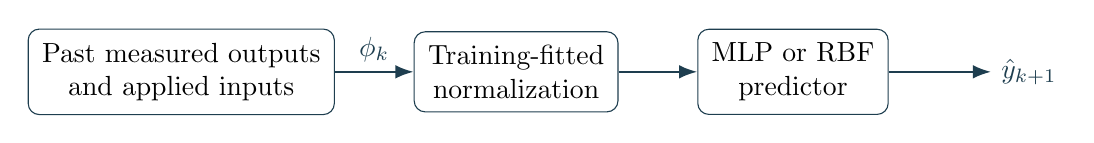
\begin{tikzpicture}[node distance=1.0cm]
\node[box] (data) {Past measured outputs\\and applied inputs};
\node[box,right=of data] (scaler) {Training-fitted\\normalization};
\node[box,right=of scaler] (net) {MLP or RBF\\predictor};
\draw[flow] (data)--node[above] {$\phi_k$}(scaler);
\draw[flow] (scaler)--(net);
\draw[flow] (net.east)--++(1.3,0) node[right] {$\hat y_{k+1}$};
\end{tikzpicture}
\end{center}
\noindent\textit{Causal regressors and fixed preprocessing are part of the model. Recursive simulation substitutes previous predictions for measured outputs; it is a different validation task.}

\subsection{Predict a dynamic relation, not a shuffled collection of rows}

A nonlinear autoregressive model with external input uses past observations and applied inputs to predict the next output. One causal choice is


\[\phi_k=[y_k,y_{k-1},u_k,u_{k-1}]^T,\qquad \hat y_{k+1}=f_\theta(\phi_k).\]

The regressor timing must be causal. Randomly shuffling heavily overlapping windows before splitting can place nearly identical trajectories in both training and testing. Split trajectories first, then construct lagged windows inside each partition. Save scaling parameters, random seed, architecture, weights and the complete data protocol.


\subsection{Four network families address different tasks}

A perceptron computes a binary decision from $\operatorname{sign}(w^Tx+b)$ and updates the separating hyperplane on classification mistakes. It is a useful diagnostic classifier for linearly separable conditions, not a continuous process simulator. An MLP composes affine maps and nonlinearities; for one hidden layer, $h=\tanh(W_1\phi+b_1)$ and $\hat y=W_2h+b_2$. Backpropagation differentiates the loss through both layers. Regularization, early stopping and independent validation limit overfitting but do not certify extrapolation.


An RBF network uses local responses $\psi_j(\phi)=\exp[-\|\phi-\mu_j\|^2/(2\sigma_j^2)]$ and a linear output. For fixed centers/widths, ridge regression determines output weights from $(\Psi^T\Psi+\alpha I)w=\Psi^TY$. Poorly placed centers can leave important operating regions unsupported. A self-organizing map (SOM) updates a best-matching unit and its neighbors, $m_j^+=m_j+\eta h_{j,j^*}(x-m_j)$. It organizes operating regimes without supervised target values; a small map distance is not a fault label or a probability.


\subsection{Accuracy is a property of the validation experiment}

Report one-step and recursive simulation errors, operating-range coverage, residual structure and behavior under changed initial conditions. Normalize errors with a declared physical scale. Preserve the physical concentration interval and compare against the linear identification baseline: a larger network is useful only if it answers a limitation the baseline actually has. Bootstrap or repeated-seed comparisons should resample whole independent runs where temporal correlation matters.


\subsection{Use a learned model in control with explicit safeguards}

A neural predictor can replace a prediction model inside MPC, or a differentiable inverse can propose an input. For a locally monotone model, a bounded Newton step is $u^+=u-\gamma(\hat y^+(u)-r)/(\partial\hat y^+/\partial u)$. A small or wrong-sign derivative makes this unreliable. Enforce actuator limits, restrict the search to supported inputs, test the candidate against a known model/constraint layer, and retain a validated fallback. Direct inverse learning can be ill-posed when different inputs produce the same output or when unobserved states matter. Good training error does not establish closed-loop stability.

\clearpage\section{Unit 07: Evolutionary optimization and controller tuning}
\textbf{Prerequisites:} Units 02, 04 and 06; random sampling, objective functions and constrained experiment design.

\subsection{Encode a controller and an experiment together}

A genetic algorithm searches a population of candidate parameters through selection, crossover and mutation. For PI tuning the chromosome may encode $(K_p,K_i)$; for multivariable MPC it may encode prediction horizon and positive input/output weights. Bounds and units are part of the representation. A chromosome is not a controller until the decoding, simulation protocol, constraints and cost are defined.


For a $b$-bit unsigned integer $q$, a parameter in $[l,h]$ is $\theta=l+(h-l)q/(2^b-1)$. Binary encoding creates quantization and bit-level neighborhoods that may differ strongly from physical distance. Real encoding avoids that quantization but still needs a documented crossover and mutation distribution. Blend crossover $\theta_c=\alpha\theta_1+(1-\alpha)\theta_2$ stays inside the parental interval when $0\leq\alpha\leq1$; Gaussian mutation may leave bounds, so repair or rejection must be specified.


\subsection{Reward what matters and reject invalid trials}

One cost is $J=\mathrm{IAE}+\beta\sum_k|u_k-u_{k-1}|+\gamma\sum_k\epsilon_k^2$, where $\epsilon$ measures permitted soft violations. Normalize terms or state their units before choosing weights. Hard physical limits should be enforced or treated as candidate rejection, not hidden by an average penalty. Terminate unstable simulations using declared state/finite-value thresholds and give them a consistently poor fitness.


Tournament selection needs only an ordering, whereas fitness-proportional selection needs nonnegative appropriately scaled fitness. Elitism preserves the best observed valid candidate; it does not establish a global optimum. Count simulation evaluations, not just generations, when comparing computational budgets. Include a grid, random search or established IMC tuning baseline so improvement can be attributed to the search method rather than additional evaluation effort.


\subsection{Separate tuning scenarios from final evaluation}

Optimize against a fixed family of training trajectories, select algorithm settings using validation scenarios, then freeze the design before testing unseen disturbances and plant mismatch. Repeated seeds reveal stochastic search variability; report the distribution and all failed runs, not only the best seed. For uncertain models, use a declared robust objective such as the maximum cost across a finite scenario set; this is robustness to that tested set, not a proof for all uncertainty.


For multivariable MPC, chromosomes must retain positive weights and integer horizons. Changing a weight changes both performance and the meaning of a reported objective; compare final controllers using a common external evaluation metric. Include solve-time and feasibility effects because a long horizon that misses the deadline is not an operational improvement.

\clearpage\section{Unit 08: Integration, benchmark evidence and technical communication}
\textbf{Prerequisites:} Units 01-07; interpretation of numerical experiments and model limitations.

\subsection{A comparison is a controlled experiment}

Start by stating the plant, operating range, measured variables, actuator limits and decision question. Establish the physical and linear identification baselines before adding neural or fuzzy components. Freeze a shared experiment contract: sample interval, numerical solver and tolerance, initial state, reference, disturbances, noise realization, controller initialization and failure policy. Keep synthetic outputs distinct from measured records. A simulation-based controller study is evidence about its declared model and scenarios.


Use the supplied integrated syllabus as a non-official study framework. The three proposed practical blocks become one connected project: identify and tune a baseline; compare alternative structures and MPC; then add an intelligent method and test its incremental value. Do not give every method a different experiment merely because one plot looks better.


\subsection{Match the article's model identity before its score}

Kroll and Schulte's article provides a benchmark survey, not a single self-contained software package. Its sections include artificial SISO and MIMO identification models; data repositories; an inverted pendulum; throttle; pneumatic actuation; hydrostatic transmission; three tanks; a bioreactor; a chemical CSTR; a binary distillation column; the ALSTOM gasifier; wind-turbine models; and the Tennessee Eastman process. Some examples specify equations; others require external data, maps, parameter choices or full reference simulators.


Record the section, equation/model variant, source version, parameters, units and any closure added by the implementation. An educational closure can illuminate a mechanism, but its results do not reproduce an external industrial benchmark. Missing physical functions must remain a visible dependency rather than be replaced by an arbitrary function with the original benchmark's name. The repository's benchmark inventory is the authority for implemented versus externally dependent cases.


\subsection{Evaluate performance and limitations jointly}

Prediction metrics include maximum absolute error, SSE, RMSE, VAF and $R^2$. VAF uses residual variance while $R^2$ uses residual squared magnitude, so a constant bias can leave VAF deceptively high. For constant targets, denominator-based metrics may be undefined; report absolute errors rather than inventing a finite score. Control metrics include IAE/ISE, peak error, settling under a stated band/dwell rule, applied effort, total variation, saturation and violations. Analyze trajectories as well as aggregates.


\subsection{Communicate a reviewable conclusion}

A technical report should connect requirements, derivation, implementation, experiment, result and limitation. Include a physical equipment diagram, a control architecture diagram and axes with units. Give enough code and configuration to reproduce every reported value. State which language/runtime was actually executed. An unrun MATLAB or Simulink port must not be presented as experimentally verified merely because Python passed.


Present improvements as conditional results: for this model, this information set and these tests, the observed tradeoff was favorable. Explain failures and unsupported extrapolation. A useful next decision may be to collect a missing measurement or validate a plant parameter, rather than introduce another algorithm.
\clearpage\section{Bibliography and reading map}
The first twelve entries reproduce the bibliographic scope of the supplied integrated syllabus. Years/editions follow that source; they are not a claim that every chapter or edition was consulted. The article supplies the benchmark framework.


\noindent 1. Massa de Campos, M.; Saito, K. \emph{Sistemas inteligentes em controle e automação de processos}. Ciência Moderna, 2004.\par\smallskip

\noindent 2. Nascimento Jr., C. L.; Yoneyama, T. \emph{Inteligência artificial em controle e automação}. Blücher, 2000.\par\smallskip

\noindent 3. Nørgaard, M.; Ravn, O.; Poulsen, N. K.; Hansen, L. K. \emph{Neural Networks for Modelling and Control of Dynamic Systems}. Springer, 2009.\par\smallskip

\noindent 4. Passino, K.; Yurkovich, S. \emph{Fuzzy Control}. Pearson, 1997.\par\smallskip

\noindent 5. Vidal, Leonardo de Carvalho. \emph{Aplicação Fuzzy x PID: Técnicas de Controle em Ambientes Simulados}. 1st ed., Appris, 2015. ISBN 978-8581927800.\par\smallskip

\noindent 6. Aguirre, Luis Antônio. \emph{Enciclopédia de Automática}, vol. 1. Blücher, 2007.\par\smallskip

\noindent 7. Aguirre, Luis Antônio. \emph{Enciclopédia de Automática}, vol. 2. Blücher, 2007.\par\smallskip

\noindent 8. Camacho, E.; Bordons Alba, C. \emph{Model Predictive Control}. Springer, 2004.\par\smallskip

\noindent 9. Ljung, L. \emph{System Identification: Theory for the User}. Pearson, 1998.\par\smallskip

\noindent 10. Simões, Marcelo Godoy; Shaw, Ian. \emph{Controle e modelagem fuzzy}. 2nd ed., Blücher, 2007. ISBN 978-8521204169.\par\smallskip

\noindent 11. Skogestad, Sigurd; Postlethwaite, Ian. \emph{Multivariable Feedback Control: Analysis and Design}. 2nd ed., Wiley, 2005.\par\smallskip

\noindent 12. Tuovinen, T.; Périaux, J.; Neittaanmäki, P. (eds.). \emph{Computational Sciences and Artificial Intelligence in Industry: New Digital Technologies for Solving Future Societal and Economical Challenges}. Springer, 2022.\par\smallskip

\noindent 13. Kroll, A.; Schulte, H. Benchmark problems for nonlinear system identification and control using Soft Computing methods: Need and overview. \emph{Applied Soft Computing} 25 (2014), 496-513. DOI: 10.1016/j.asoc.2014.08.034.\par\smallskip

Suggested reading by unit: 01 (3, 9, 13); 02 (1, 6, 7); 03 (1, 11); 04 (8, 11); 05 (1, 2, 4, 5, 10); 06 (2, 3); 07 (1, 2, 12); 08 (8, 9, 11, 12, 13).

\end{document}
